\documentclass[UTF8,11pt]{ctexart}

\usepackage[margin=1in]{geometry}
\usepackage{booktabs}
\usepackage{graphicx}
\usepackage{amsmath}
\usepackage[hidelinks]{hyperref}
\usepackage{xcolor}
\usepackage{enumitem}
\usepackage{microtype}

\graphicspath{{figures/beta/}{figures/}}

\title{共识合并如何把正确的共享经验\\ 变成多智能体系统中的静默策略退化}
\author{Phase-Beta 结果章节（中文阅读版）}
\date{\today}

\begin{document}
\maketitle

\begin{center}
\fcolorbox{teal!70!black}{teal!5}{\parbox{0.94\linewidth}{%
\textbf{草稿说明。}以下数字全部来自预注册的 Phase-Beta 方案（\texttt{prereg\_phase\_beta.md}）；
判决规则在数据采集前冻结，每个判决都记录在该文档的偏离日志里。统计一律为同迷宫配对 bootstrap
（10000 次重采样，95\% 置信区间）。经验文本全部由模型生成，sanitizer 保证经验池中不含任何
研究者书写的字符串。}}
\end{center}

\begin{abstract}
我们研究多智能体 LLM 系统中的共享经验记忆是否会把局部正确的策略放大为全局退化的行为。
借助一个可控迷宫显微镜（每个动作都合法、最短路径可测），我们在预注册的实验阶梯上，
用忠实实现的 ExpeL 式经验操作和 Generative-Agents 式检索进行验证。主要发现：
(i) 在单智能体层面，忠实的经验学习不会显著改变效率主终点（归因对照）；
(ii) 在多智能体层面，注入经验会降低效率、放大循环，其中\emph{共识合并型}共享记忆产生
跨 seed 最稳健的退化，也是唯一相对私有记忆显著放大循环的写入方式；
(iii) 危害不来自读端的使用量加权检索（剂量-反应为零结果），而来自写端合并，
它把整个种群的活跃策略供给压缩了约一倍。这种失败是静默的：agent 仍然成功、从不穿墙、
也从不错误提交，却越来越多地在原地绕圈。
\end{abstract}

\section{实验阶梯与判决}

我们在生成的 $15\times15$ trap 迷宫家族（最短路径 $\geq 30$）上评测，使用局部观测、
state-guided 控制器、步数上限 120。solver 从不看到迷宫图或最短路径。各记忆条件只在
\emph{写入协议}和\emph{是否共享}上不同；reviewer 只看到 agent 日志与质量信号，看不到隐藏路径。
预先冻结的主终点是：成功路线的超额步数、循环率、多智能体 ant-mill 率。

\subsection{E1：单智能体归因对照}

在引入共享之前，先问忠实的经验学习是否会改变单智能体行为。相对无记忆基线（配对、末轮、三 seed），
无论 ExpeL 操作集写入还是 append 写入，都没有移动任何主终点：成功路线超额步数的置信区间含 0
（append $-4.74$，CI $[-14.1, +4.2]$；ops $+5.11$，CI $[-6.4, +16.3]$），循环率同样含 0。
按冻结规则这是\textbf{不通过（FAIL）}。但规定的依从性分析显示经验\emph{并未}被忽略：
记忆激活后，ops 写入让动作选择偏离控制器建议（$+0.041$，$3/3$ seed 同号），
append 写入显著降低最大重访次数。因此这个单智能体零结果是一个\emph{归因对照}：
之后任何多智能体退化都不能归因于“用了记忆”本身，只能归因于共享通道。

\subsection{E2：多智能体记忆矩阵}

我们在四智能体、$T=6$、五 seed 下比较五个条件臂，基线是只写不读、累积但从不注入经验的
\emph{frozen} 控制组。表~\ref{tab:e2} 与图~\ref{fig:fig2} 报告末轮的配对差异。

\begin{table}[h]
\centering
\caption{E2 末轮相对 frozen 的配对差异（五 seed，$n_{\text{pairs}}=240$；
成功路线超额步数会丢弃无法配对的失败路线）。$^\ast$ 表示 95\% 置信区间不含 0。}
\label{tab:e2}
\begin{tabular}{lrrrr}
\toprule
条件臂 & 成功率 & 成功路超额步数 & 循环率 & 最大重访 \\
\midrule
MAS 无记忆        & $-0.004$          & $+1.12$            & $+0.042^\ast$ & $+0.10$ \\
私有记忆          & $-0.175^\ast$     & $+7.32^\ast$       & $+0.079^\ast$ & $+1.20^\ast$ \\
共享 append       & $-0.121^\ast$     & $+2.75$            & $+0.025$      & $+0.23$ \\
共享 consolidated & $-0.171^\ast$     & $+11.84^\ast$      & $+0.138^\ast$ & $+1.68^\ast$ \\
\bottomrule
\end{tabular}
\end{table}

由此得到三点。第一，多智能体执行本身不病态：MAS 无记忆在效率与成功率上与 frozen 一致，
仅有轻微循环上升（$+0.042$，CI $[0.008, 0.075]$）。第二，\textbf{共识合并型共享记忆满足
全部预注册退化判据}：成功路超额步数 $+11.84$（CI $[7.66, 16.02]$），$5/5$ seed 同号
且后面的 seed 效应\emph{更大}；循环率 $+0.138$（CI $[0.092, 0.188]$）；成功率 $-0.171$。
第三，广义风险来自主动注入而非仅仅共享——私有记忆也退化——所以我们直接检验共享特异性。

\paragraph{共享 vs 私有的边界。}图~\ref{fig:fig2b} 把共享臂与\emph{私有}基线对比。
效率维度的分离不显著（consolidated vs 私有的成功路超额步数 $+0.87$，CI $[-4.29, +6.15]$），
但循环放大显著：consolidated 的循环显著多于私有（$+0.058$，CI $[0.008, 0.113]$），
而 append 反而更\emph{少}循环。因此诚实的表述是：共识合并特异性地相对私有放大了循环；
我们\emph{不}声称共享在效率上普遍坏于私有。

\subsection{E3：读端剂量-反应为零结果}

如果危害在读端——agent 越来越多地检索少数高票经验——那么在 Generative-Agents 式打分里
提高 importance 权重 $\lambda$ 应当加深退化。事实并非如此。在 append 臂上扫
$\lambda\in\{0,0.5,1\}$（三 seed，$T=6$），$\lambda{=}1$ 相对 $\lambda{=}0$ 的成功路超额步数
配对差为 $+1.69$（CI $[-4.26, +7.61]$），循环率 $+0.049$（CI $[0.000, 0.104]$），
且末轮检索熵关于 $\lambda$ 非单调（$0.833/0.826/0.845$）。读端使用量加权反馈假设被
\textbf{判伪}；我们如实报告为一个干净的零结果。

\subsection{机制：写端策略供给压缩}

对同一批 E2 run 的离线审计把集中定位在\emph{写}端（图~\ref{fig:fig3}）。相同设置下，
consolidated 池收敛到 $14.2$ 条，全部轮次实际注入的不同经验只有 $11.0$ 条；
而 append 池长到上限（$80$）、注入 $25.4$ 条不同经验，私有注入 $37.6$ 条。
共识合并把种群的活跃策略供给相对 append 压缩了约 $2.3\times$。top-1 检索份额随之上升，
但这是池更小的后果而非独立通道；承重证据是池大小与不同注入数这两个直接计数。

\subsection{E4：长反馈链压力测试（探索性）}

为了检验写端危害在更长反馈链下是饱和、加深还是自愈，我们把四智能体共享臂延长到 $T{=}10$
（三 seed，heldout 12，含 frozen 与共享 append 对照；按预注册为非 gate 探索性实验）。
相对 frozen，共享 consolidated 的退化在所检验的每个检查点（$t=3,6,9$）都存在且没有收窄：
成功率差为 $-0.174$、$-0.146$、$-0.257$（置信区间全部不含 0），循环率差为 $+0.083$、
$+0.083$、$+0.118$（置信区间全部不含 0），末轮是三点中最差的一点。更严格的组内检验——
比较每个条件自身末三轮与前三轮（排除暖启动轮 $t{=}0$）——发现 consolidated 在全部六项
终点上都没有显著的自身趋势：差距是早期就打开的，随后停在一个带噪声的高位平台，
而非可证实地持续加深。相反，append 臂在同样的长链上呈现显著的组内\emph{改善}
（cost ratio $-0.079$、超额步数 $-3.50$、stagnation $-0.026$、最大重访 $-0.340$，
置信区间全部不含 0），到 $t{=}9$ 时其 cost ratio、超额步数、最大重访均显著优于
frozen——与“策略供给未被压缩的写协议能持续从积累中获益”这一判断一致。
把共享 consolidated 的组内趋势按 seed 拆开，会暴露出被均值掩盖的异质性。
seed 1 是唯一在 late-vs-early 成功率比较中显著下降的 seed（$-0.097$，置信区间不含 0），
但它的逐轮轨迹以震荡为主，并非单调下滑。seed 2 的逐轮轨迹最严重，末轮成功率降至
$0.17$、循环率升至 $0.46$，但其 late-vs-early 成功率置信区间仍包含 0；seed 0
则没有显著下降。因此“组内无显著进一步漂移”这个判决是一个混合种群上的均值，
而不是“每个实例都同样稳定”的证据；我们把这一点标记为外部效度后续验证的目标，
而非已定论的主张。

\section{这种失败是静默的}

图~\ref{fig:fig1} 展示机制示意与一个从 run 中挖出的案例：同一张 heldout 迷宫、同一 agent、
末轮，最短路径 38 步。随着写入协议合并，路线单调退化——frozen 39 步（重访 1 次），
私有 47 步（4 次），共享 append 55 步（9 次），共享 consolidated 73 步、cost 1.92、
对同一格重访 11 次并被检出循环——但每条路线都合法、每个臂都到达终点。
这就是 ant-mill 签名：不是学到了假知识，而是一个局部合理的纠偏信号，经共识写入强化后，
复合成了全局浪费的循环。

\clearpage
\section{结论一览}

\begin{itemize}[leftmargin=1.4em]
\item 单智能体忠实经验学习不移动主终点（归因对照；E1）。
\item 多智能体经验注入降低效率、放大循环；共识合并是跨 seed 最稳健的退化臂（E2）。
\item 相对私有记忆，共享特异性效应是循环放大，而非普遍的效率差距（E2 边界）。
\item 危害不来自读端使用量加权检索（零剂量-反应；E3），而来自压缩活跃策略供给的
写端合并（机制审计）。
\item 延长到更长反馈链（$T{=}10$）后，consolidation 的危害持续存在、在种群层面没有
可证实的进一步加深。按 seed 拆分后，一个 seed 呈现显著的组内下降，另一个 seed
轨迹更极端但置信区间仍无定论（E4，探索性）。
\end{itemize}

% ---------------------------------------------------------------- figures
\begin{figure}[p]
\centering
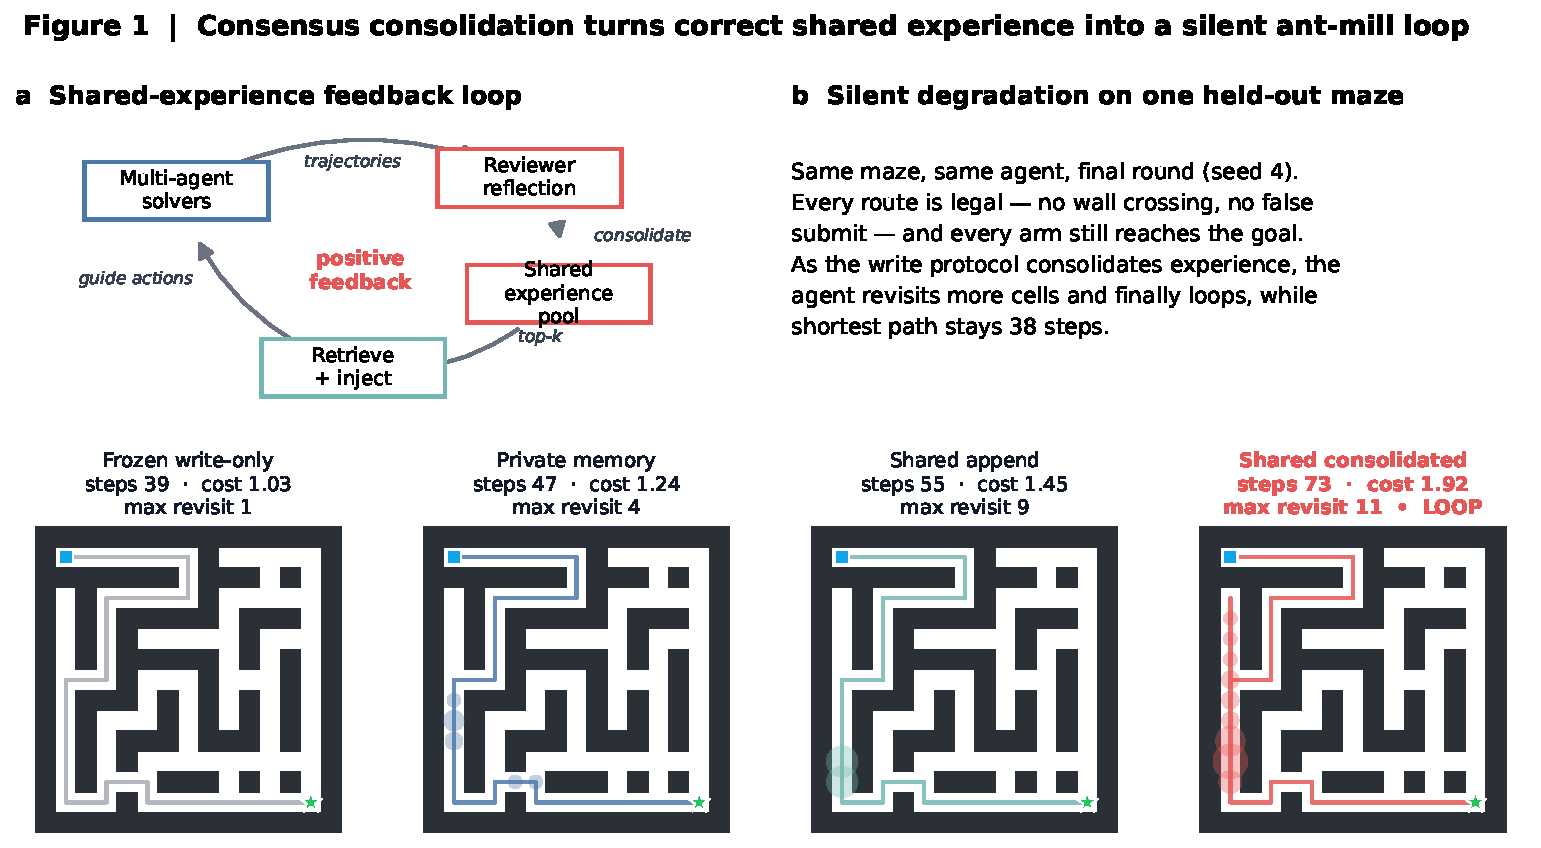
\includegraphics[width=\linewidth]{figure1_mechanism.pdf}
\caption{\textbf{机制显微镜与一个静默退化案例。}
(a) 共享经验反馈环：solver 轨迹被反思进共享池，由 LLM 发出的操作合并，检索 top-$k$，
再作为指导注入回来——一个正反馈循环。(b) 同一 heldout 迷宫与 agent，末轮，最短路径 38。
重访热度（阴影圆点）随写入协议合并而增长，在共享 consolidated 记忆下形成静默循环，
而每条路线始终合法且成功。}
\label{fig:fig1}
\end{figure}

\begin{figure}[p]
\centering
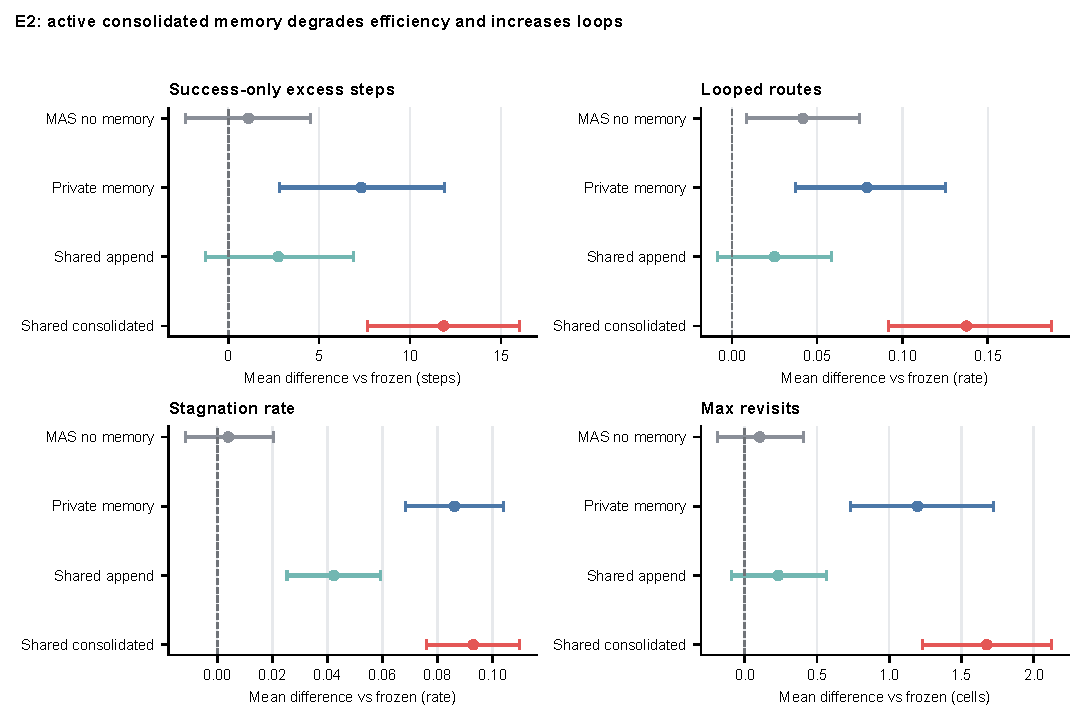
\includegraphics[width=\linewidth]{figure2_e2_main.pdf}
\caption{\textbf{E2 主结果：相对 frozen 只写记忆的配对差异}（五 seed，末轮）。
点为均值差，误差棒为 95\% bootstrap 置信区间，虚线为 0。共享 consolidated（红）在四个终点上
全部退化且效应最大；MAS 无记忆（灰）除轻微循环上升外都压在 0 线。}
\label{fig:fig2}
\end{figure}

\begin{figure}[p]
\centering
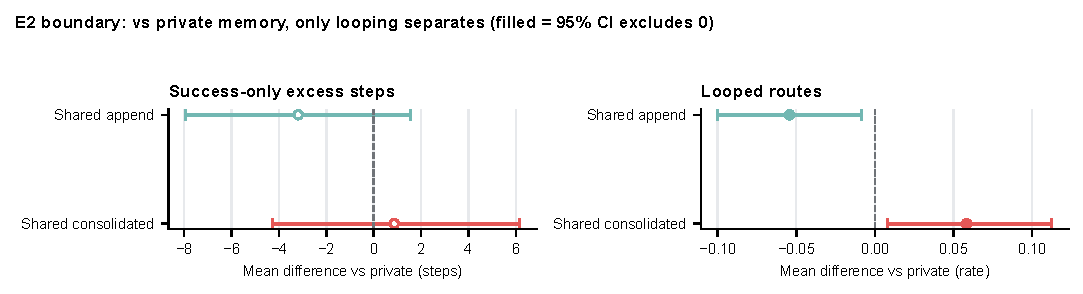
\includegraphics[width=\linewidth]{figure2b_shared_vs_private.pdf}
\caption{\textbf{E2 边界：共享臂相对私有基线。}
实心点表示置信区间不含 0。只有循环把共享 consolidated 与私有分开（$+0.058$，CI $[0.008, 0.113]$）；
效率对比不显著，且共享 append 实际上比私有更少循环。}
\label{fig:fig2b}
\end{figure}

\begin{figure}[p]
\centering
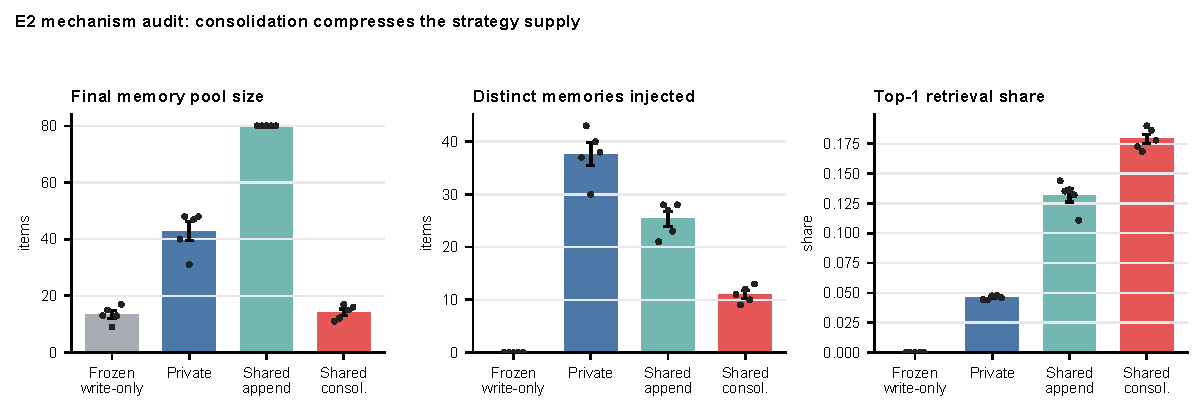
\includegraphics[width=\linewidth]{figure3_write_side_compression.pdf}
\caption{\textbf{机制审计：合并压缩了策略供给。}
五 seed 下的最终池大小、实际注入的不同经验数、top-1 检索份额（散点）。
共识合并保持小池、注入最少的不同策略、并集中检索；左中两格的直接计数承担因果主张。}
\label{fig:fig3}
\end{figure}

\end{document}
